\chapter{Marco Teórico}

\section{Internet de las Cosas}

El Internet De las Cosas (IoT por sus siglas en inglés - Internet of Things) es un concepto que busca la interconexión de objetos y dispositivos con la capacidad de ser identificados de manera única en la amplia red de internet, de tal manera que cada uno de ellos tenga una función dentro un sistema a pequeña o gran escala, ya sea generar datos, recopilar datos o incluso visualizar y manipular un entorno de aplicación, sea una casa, restaurante, supermercado, fabrica e incluso una ciudad entre la infinidad de escenarios posibles, dentro de los cuales existen interacciones de carácter humano- maquina, es decir, un usuario accediendo a una interfaz que le permita conocer el estado de su entorno en cuestión y la interacción máquina-máquina, la cual puede darse entre un sensor recopilando información, el cual a través de un sistema de mando tome una decisión inteligente, tal como activar un sistema de riego con poca humedad o cerrar una ventana en presencia de lluvia.\cite{TechT2017} \\

A pesar de ser un concepto concebido alrededor de los años 80, IoT no ha llegado a un consenso o un estándar para su aplicación, es por eso que en la actualidad existe una gran cantidad de investigaciones y aplicaciones comerciales con diferentes enfoques y tecnologías, facilitando así que el desarrollo tecnológico tenga un avance global, a la vez que el Internet De las Cosas genera datos para uso estadístico o comercial, permitiendo también conocer comportamientos más precisos de un sistema, con lo cual hace posible pensar en estrategias para reducir perdidas y costos.\cite{Asthon2009} \\


\subsection{Plataforma Heroku}

Heroku es una PaaS (Plataforma Como Servicio - Platform as a Service) que permite el despliegue de una aplicación web sin que el programador se preocupe por cuestiones de infraestructura, administrar servidores, bases de datos, entre otras características de software, pues este solo requiere conocer detalles como el lenguaje de backend a utilizar y  la base de datos. Cada aplicación puesta en marcha sobre esta plataforma esta almacenada en su repositorio, pues esta basada en un sistema gestionado por contenedores.\cite{Hero}\\


\subsection{Framework Laravel}

Laravel es un framework de código abierto fácil de asimilar para lenguaje PHP, usado para el desarrollo de aplicaciones web tiene como objetivo aumentar la comodidad al desarrollarlas, contando con una sintaxis expresiva y elegante facilita tareas comunes presentes en la mayor parte de proyectos de este tipo, tales como autentificación, enrutamiento, sesiones y almacenamiento en caché. \\

“Laravel es accesible, pero potente, y proporciona potentes herramientas necesarias para aplicaciones grandes y robustas. Una magnífica inversión de contenedores de control, un sistema de migración expresivo y un soporte de prueba de unidades estrechamente integrado le brindan las herramientas que necesita para construir cualquier aplicación'' \cite{Lara}.\\

Algunas características generales de este framework son:



\begin{itemize}
	\item Sistema de ruteo, también RESTful
	\item Blade, Motor de plantillas
	\item Peticiones Fluent
	\item Eloquent ORM
	\item Basado en Composer
	\item Soporte para el caché
	\item Soporte para MVC
	\item Usa componentes de Symfony
	\item Adopta las especificaciones PSR-2 y PSR-4	
\end{itemize}

\subsection{HTTP}

El protocolo de transferencia de hipertexto (HTTP) es un protocolo de la capa de aplicación en el modelo OSI, usado para transmitir documentos hipermedia como HTML. Diseñado con el propósito de la comunicación entre navegadores y servidores web, no obstante, puede operar con otros propósitos. HTTP sigue un modelo clásico de cliente-servidor, con un cliente que abre una conexión y realiza una petición a la espera de respuesta. HTTP es un protocolo sin estado, significa que el servidor no conserva ningún dato entre dos solicitudes. Para realizar las peticiones, este protocolo cuenta con diferentes metodos \cite{HTTP}.

\paragraph{Métodos de solicitud HTTP:}

HTTP define un conjunto de métodos de solicitudes para indicar la acción deseada que se realizará a un recurso determinado. Aunque pueden ser sustantivos, estos métodos algunas veces se denominan verbos HTTP. Cada uno de ellos implementa una semántica diferente, pero algunas características comunes son compartidas por un grupo de ellos \cite{HTTPM}.\\

\begin{itemize}
	\item GET: este método solicita una representación del recurso especificado. Las peticiones que lo usan, solo deben regresar datos.
	\item HEAD: este método solicita una respuesta igual a una peticion GET, pero sin el cuerpo de la respuesta.
	\item POST: se usa para enviar una entidad al recurso especificado, causando a menudo un cambio en el estado o efectos secundarios en el servidor.
	\item PUT: reemplaza todas las representaciones actuales del recurso destino con la la petición de carga útil.
	\item DELETE: esta petición elimina el recurso especificado.
	\item CONNECT: establece un túnel para el servidor identificado por el recurso de destino.
	\item OPTIONS: se usa para describir las opciones de la comunicación para el recurso destino.
	\item TRACE: realiza una prueba de mensaje loop-back a lo largo de la ruta del recurso de destino. 
	\item PATCH: se usa para realizar modificaciones parciales a un recurso.
\end{itemize}

\subsection{JSON}

JSON (JavaScript Object Notation – Notacion de Objetos de JavaScript) es un formato basado en texto para representar datos e intercambiarlos, comúnmente utilizado en aplicaciones web pues para las maquinas resulta simple interpretando y generarlo, al igual que para los humanos es cómodo leerlo y escribirlo. JSON no tiene dependencia directa con el lenguaje de programación utilizado, no obstante su sintaxis comparte convenciones conocidas en  lenguajes de programación como C, C++, Java, JavaScript, Python, entre otros, lo cual lo hace ideal para cumplir su objetivo. \\

``JSON está constituído por dos estructuras:

\begin{itemize}
	\item Una colección de pares de nombre/valor. En varios lenguajes esto es conocido como un objeto, registro, estructura, diccionario, tabla hash, lista de claves o un arreglo asociativo.
	\item Una lista ordenada de valores. En la mayoría de los lenguajes, esto se implementa como arreglos, vectores, listas o secuencias.''\cite{JSON}.
\end{itemize}


\subsection{Base de Datos}

Desde un punto de vista informático, una base de datos es un sistema estructurado de información almacenada y relacionada entre sí, la cual puede ser visualizada por medio de un acceso directo a ellas o teniendo un conjunto de programas o tareas encargadas de su gestión y/o modificación.\\

Las bases de datos están compuestas por una o más tablas donde se guarda la información ordenadamente en filas y columnas, donde se encuentra cada elemento que queramos guardar junto con su correspondiente registro \cite{DB}.\\ 

Para la gestión de datos es muy común encontrar las funciones básicas de crear, leer, actualizar y borrar (CRUD), con la finalidad de que el usuario final pueda acceder a estos sin necesidad de realizar peticiones directamente a la base de datos, sino en una interfaz gráfica (GUI).\\

\section{Smart House}

El concepto de Smart House implica tres características básicas. En primer lugar, el monitoreo a través de redes de sensores para obtener información sobre la casa y sus residentes. En segundo lugar, los mecanismos que controlan el uso de la comunicación entre dispositivos con el fin de permitir la automatización y el acceso remoto. Por último, las interfaces de usuario, como los teléfonos inteligentes y las computadoras que permiten a los usuarios especificar las preferencias, así como presentar información a las personas acerca de estas. \\

Smart House es un entorno que tiene sistemas sofisticados a través de los cuales se pueden controlar algunos de los objetos de la casa, como luces, puertas, ventanas, además puede racionalizar el consumo de energía, entre otras funciones mediante el uso de sensores. Básicamente, uno de los beneficios más importantes del uso de la tecnología en las casas, es la prestación de servicios a las personas.\cite{Howedi2016} 

\section{Hardware}

\subsection{ESP-WROOM-32}

Este es un potente módulo MCU Wi-Fi + BT + BLE creado con un enfoque hacia aplicaciones de IoT, esta también dirigido e implementado en una amplia variedad de proyectos con tareas simples o más exigentes gracias a sus amplias capacidades y alcance físico por su conexión Wifi a internet, además de garantizar un bajo consumo de potencia y un reducido tamaño según se observa en la Figura \ref{fig:esp32-wroom-s32-00}. La corriente de reposo del chip ESP32 es inferior a 5 $\mu$A, lo que lo hace adecuado para aplicaciones de electrónica con batería y portátiles.\\

El chip en cuestión está diseñado para ser adaptable y tener escalabilidad. Su CPU cuenta con dos núcleos, los cuales pueden ser administrados y controlados individualmente, modificación también su frecuencia de reloj en un rango entre 80MHz y 240MHz, con velocidades de datos de hasta 150Mbps y una potencia de salida de 20.5 dBm en la antena. Además de contar con múltiples periféricos, tales como sensores hall, interfaz de tarjeta SD, soporte para Ethernet, SPI de alta velocidad, UART, I2C, entre otras.\\

El sistema operativo elegido para ESP32 es freeRTOS con LwIP; TLS 1.2 con aceleración de hardware está integrado también, además se admite la actualización segura (cifrada) a través del aire (OTA), de modo que los desarrolladores puedan actualizar continuamente sus productos incluso después de su lanzamiento.\cite{EW32}


\begin{figure}[H]
	\centering
	\caption[ESP WROOM 32.]{ESP WROOM 32. Tomado de: \cite{ESPIMG}}
	\label{fig:esp32-wroom-s32-00}
	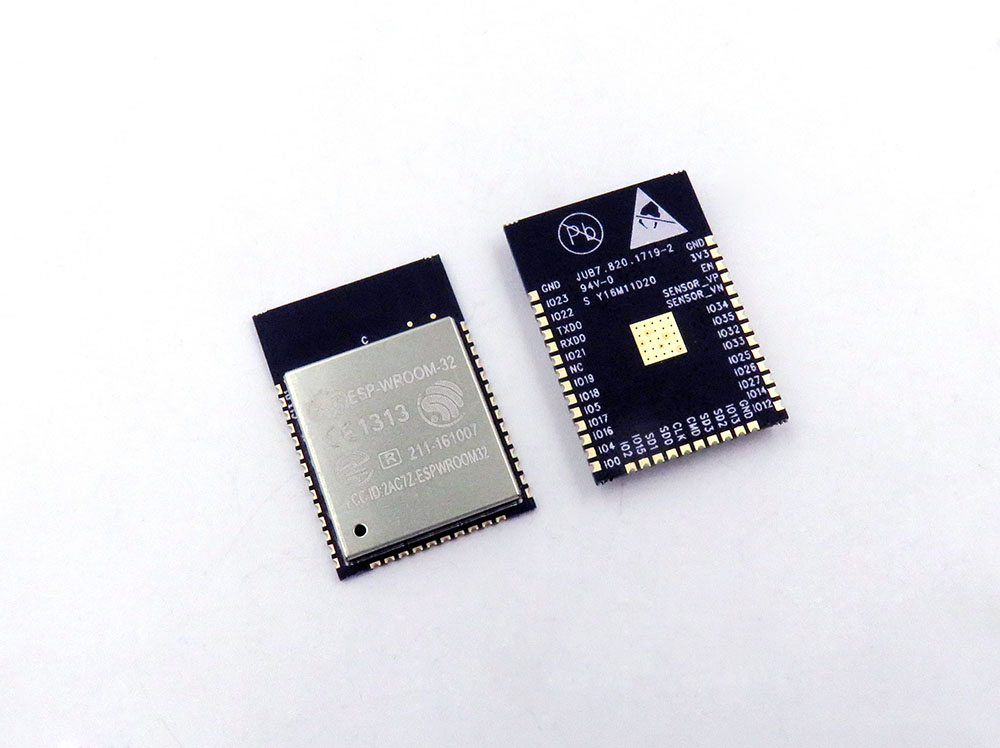
\includegraphics{Imagenes/esp32-wroom-s32-00}
\end{figure}

\subsection{Corriente Alterna (AC)}

La corriente alterna, presenta un flujo de electrones en intervalos regulares o en ciclos. Normalmente generadas en centrales eléctricas para hacer que fluya a través de las líneas eléctricas y finalmente llegando a entornos como hogares, siendo usados por los usuarios a través de enchufes sobre la pared. Esta corriente eléctrica viene con un estándar utilizado en EE.UU. a 60Hz, mientras que en Europa y en muchos lugares del mundo se manejan frecuencias de 50Hz. \cite{Cor}

\subsection{Corriente Directa (DC)}

La corriente directa tiene un flujo de electrones constante, tal como la energía eléctrica de una batería en una linterna o cualquier otro aparato de este estilo. En contraste con la corriente alterna, la perdida de energía al transportarla a largas distancias es mucho menor, además de que su cambio de voltaje resulta relativamente más económico. \cite{Cor}\\

\subsection{Control de potencia AC por ángulo de fase}

Dispositivos como TRIAC y SCR facilitan el uso de técnicas para controlar la potencia de una carga mediante la manipulación del voltaje promedio, modificando el ángulo de fase que suministra la corriente alterna de la red eléctrica. Esta técnica es utilizada en aplicaciones como intensidad lumínica, control de temperatura, regulación de velocidad en motores, entre otras.\cite{CEKIT}\\

Se puede asumir que un TRIAC	conectado en serie a el dispositivo, se comporta como un interruptor que se activa o desactiva con la presencia o ausencia de una corriente Ig en la compuerta (G). En la Figura \ref{fig:triacgraph} se observa el control de una onda seno con un periodo de 360 grados, donde la parte (a) representa la tensión a través del TRIAC y en la parte (b) la tensión sobre la carga; se observa allí que el TRIAC permanece como un circuito abierto en los primeros 45 grados de cada semiciclo, pues este es el ángulo donde comienza la conducción, conocido también como ángulo de disparo, punto a partir del cual la carga adquiere todo el voltaje de la red. \cite{CEKIT}.\\


\begin{figure}[H]
	\centering
	\caption[Representación gráfica del ángulo de disparo y de conducción del TRIAC y de la carga.]{Representación gráfica del ángulo de disparo y de conducción del TRIAC y de la carga. Tomado de: \cite{CEKIT}.}
	\label{fig:triacgraph}
	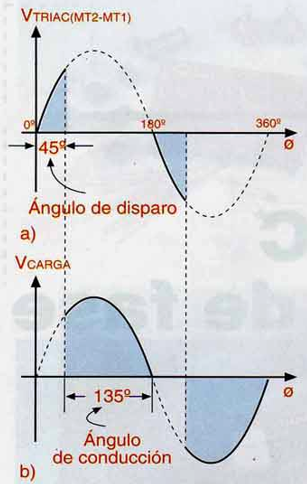
\includegraphics[width=0.3\linewidth]{Imagenes/TRIAC_graph}
\end{figure}

\subsection{Control de Cargas DC}

Los transistores como switch permiten controlar las cargas de corriente continua con ayuda de una señal PWM que los activa o desactiva. Las cargas de corriente continuas típicas como los motores y LED's, a parte de poder funcionar en dos estados, encendido y apagado, pueden se controladas mediante la modulación por ancho de pulso (PWM), ya que al variar el ancho de pulso de la señal eléctrica se varia la cantidad de energía entregada a la carga, por ejemplo, si es un LED el cambio se refleja en su intensidad lumínica y si es un motor DC cambia su velocidad de giro \cite{PWM}. Este control se produce gracias a que en esta modulación se modifica su ciclo útil, cambiando el tiempo en que la señal eléctrica se encuentra en alto durante un periodo, por lo tanto si el ciclo útil es del 10\% el poder entregado es poco, en comparación, con un ciclo útil del 50\% o 100\% conforme se observa en la Figura \ref{fig:pwm-duty-800x396}.

\begin{figure}[H]
	\centering
	\caption[Ciclo Útil PWM.]{Ciclo Útil PWM. [Imagen Propia] }
	\label{fig:pwm-duty-800x396}
	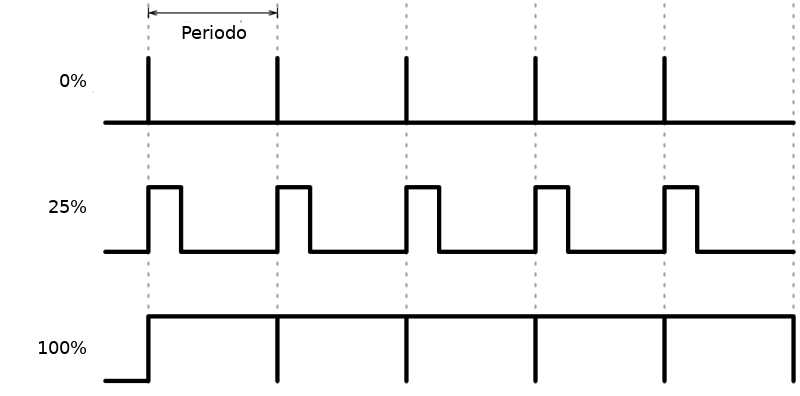
\includegraphics[width=0.5\linewidth]{Imagenes/pwm}
\end{figure}


\subsection{I2C}

I2C, también conocido como IIC ó TWI – Two Wire Interface es un protocolo de comunicación serial, el cual define una trama de datos y la conexión física de hasta 127 dispositivos esclavos con dos líneas o cables de comunicación, SDA y SCL, con velocidades de 100, 400 y 1000 Kbits/s. \cite{I2C} \\

\subsection{Sensores}\label{sec:sensors}

\subsubsection{Módulo GY-30}

El modulo sensor digital GY-30 BH1750FVI ilustrado en la Figura \ref{fig:gy-30} permite tomar una medición de la intensidad de luz ambiente o luz visible, contando con un ADC de 16bits y comunicación por medio del protocolo I2C, de tal manera que puede ser implementado en la mayoría de micro controladores. Este sensor arroja valores en la unidad Lux (Lumen /m$^2$ ), la cual es una unidad estándar para esta magnitud, teniendo un rango de operación entre 1 y 65353 lx.\cite{GY30}\\

\begin{figure}[H]
	\centering
	\caption[Módulo GY-30.]{Módulo GY-30. Tomado de: \cite{GY30}}
	\label{fig:gy-30}
	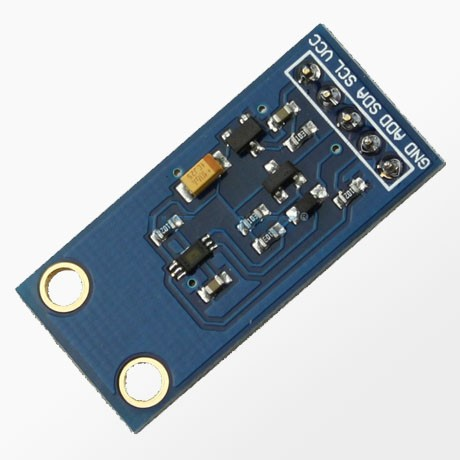
\includegraphics[width=0.4\linewidth]{Imagenes/gy-30}
\end{figure}

\subsubsection{Temperatura y Humedad DHT11}

El sensor digital DHT11 permite medir temperatura y humedad a un costo bajo, se vale de un sensor capacitivo de humedad y un termistor para medir el aire de su entorno. Este sensor conlleva una utilización sencilla, a pesar de esto requiere una cuidadosa sincronización al realizar una medida, pues este tiene un tiempo mínimo de actualización cada 2 segundos. \cite{DHT11}\\

\begin{figure}[H]
	\centering
	\caption[Sensor de temperatura y humedad DHT11.]{Sensor de temperatura y humedad DHT11. Tomado de: \cite{DHT11}}
	\label{fig:dht11}
	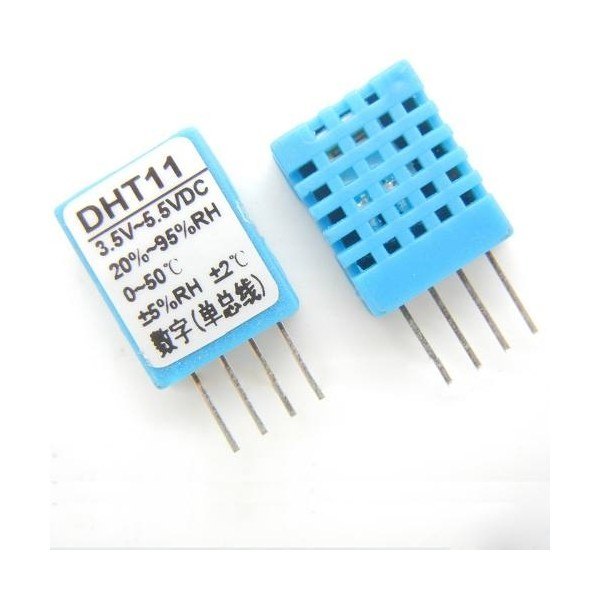
\includegraphics[width=0.4\linewidth]{Imagenes/dht11}
\end{figure}


\subsubsection{Módulo sensor de calidad de aire MQ-135}

La serie MQ de sensores de gas son sensores analógicos, por lo cual son fáciles de implementar con cualquier microcontrolador que posea un conversor analógico digital (ADC) adecuado. Estos detectores son electroquímicos y cambian su resistencia con la exposición a determinados gases, internamente poseen un calentador que se encarga de aumentar la temperatura interna para que el sensor pueda reaccionar con los gases provocando un cambio de valor en la resistencia, su estructura interior se puede observar en la Figura \ref{fig:estructura-del-sensor-mq}.\cite{MQ1}

\begin{figure}[H]
	\centering
	\caption[Estructura del sensor MQ.]{Estructura del sensor MQ. Tomado de: \cite{MQ1}}
	\label{fig:estructura-del-sensor-mq}
	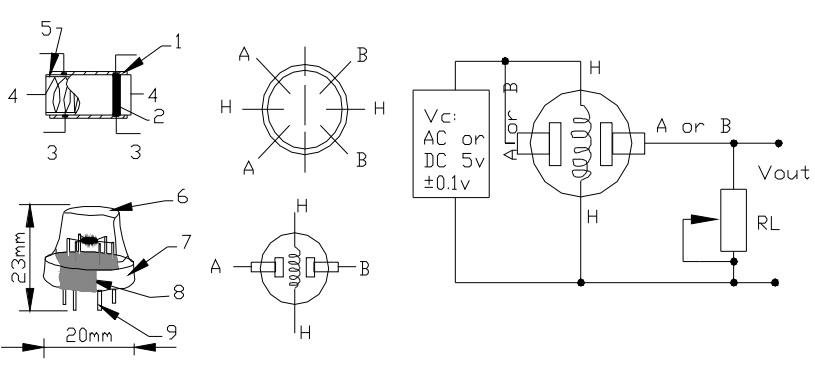
\includegraphics[width=0.7\linewidth]{Imagenes/Estructura_del_sensor_MQ}
\end{figure}

El Sensor Calidad Aire MQ135 se utilizan en equipos de control de calidad del aire a edificios y oficinas, son adecuados para la detección de NH3, NOx, alcohol, benceno, humo, CO2, etc; además de que estos sensores vienen en módulos como se observa en la Figura \ref{fig:sensor-calidad-aire-mq135}, lo que facilita su uso, simplemente se debe conectar al microcontrolador sin necesidad de utilizar algún circuito de acople. \cite{MQ1}

\begin{figure}[H]
	\centering
	\caption[Módulo sensor de calidad de Aire MQ-135.]{Módulo sensor de calidad de Aire MQ-135. Tomado de: \cite{MQ1}}
	\label{fig:sensor-calidad-aire-mq135}
 	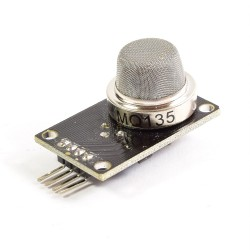
\includegraphics[width=0.35\linewidth]{Imagenes/sensor-calidad-aire-mq135}
\end{figure}

Este sensor es sensible en similar proporción a los gases mencionados, con lo que se puede determinar si el aire está limpio o si existe presencia de algún gas nocivo.\\

Los datos de salida de este sensor no son valores absolutos, simplemente proporciona una salida analógica que se debe monitorear y ser comparada con los valores típicos proporcionados en la hoja de datos.\cite{MQ2}

\subsubsection{Sensores de Estado}

Los sensores de estado describen si la variable está en alto (1) o en bajo (0), para estos detectores se tienen variables típicas, como el estado de una puerta o una ventana (abierta o cerrada), la lluvia, el movimiento.

\paragraph{Módulo detector de lluvia: }

Es un módulo relativamente simple que consiste en una serie de pistas conductoras organizadas de forma paralela e impresas sobre una placa de baquelita como se observa en la Figura \ref{fig:yl-83}. La separación entre sus caminos es muy pequeña, con el fin de crear un corto circuito cada vez que las pistas se mojan, ya que es un circuito abierto y el agua hace que se cree un camino de baja resistencia entre las pistas que tienen diferente potencial (Vcc-GND). La corriente que fluye a través de estas pistas se ve limitada por resistencias de 10K$\Omega$ en cada conductor, lo que impide que el corto circuito que se genera cuando se moja la placa vaya a estropear el micro controlador.\cite{LLU}

\begin{figure}[H]
	\centering
	\caption[Sensor de Lluvia.]{Sensor de Lluvia. Tomado de: \cite{LLU}}
	\label{fig:yl-83}
	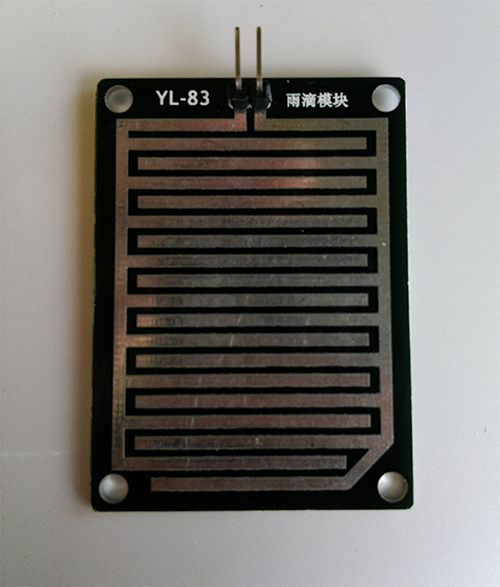
\includegraphics[width=0.35\linewidth]{Imagenes/YL-83}
\end{figure}

El circuito de control es el que posee las resistencias limitadoras de corriente y es el encargado de alimentar el módulo de la Figura \ref{fig:yl-83}. Como se observa en la Figura \ref{fig:yl-831} tiene un amplificador operacional, específicamente el circuito integrado LM392. Este se ocupa de amplificar el pequeño diferencial de voltaje que se produce cuando una gota de agua cae sobre las pistas del módulo. Aquí es donde se genera la señal de salida que puede ser del tipo analógica o digital. La señal digital oscilará entre los valores HIGH y LOW dependiendo de si hay agua o no sobre las pistas de la placa.\\

La salida analógica entregará un nivel de voltaje que variará dependiendo de la cantidad de agua que haya sobre el módulo.\cite{LLU}\\

\begin{figure}[H]
	\centering
	\caption[Módulo de sensor de lluvia.]{Módulo de sensor de lluvia. [Imagen Propia]}
	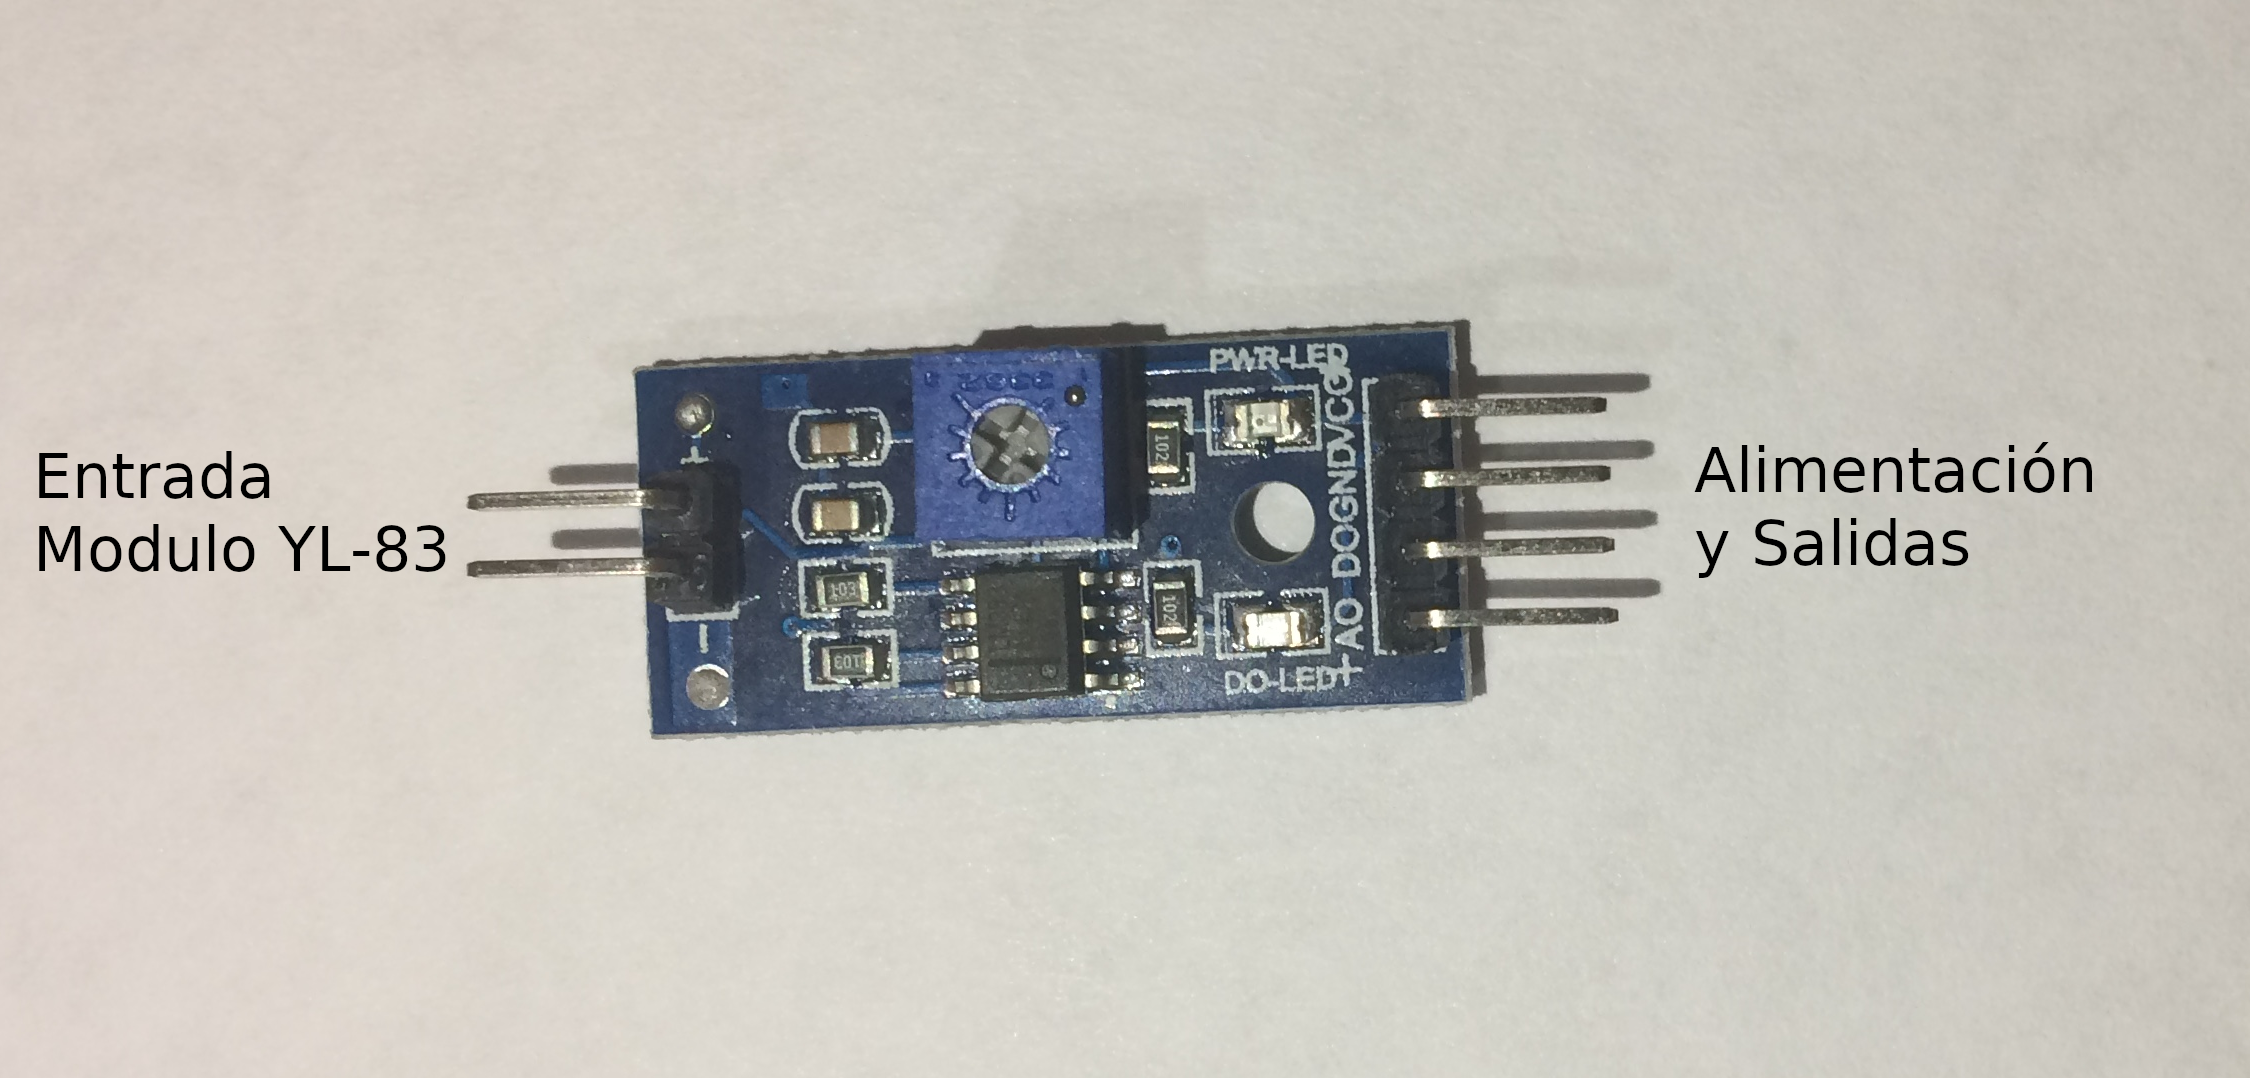
\includegraphics[width=0.5\linewidth]{Imagenes/YL-831}
	\label{fig:yl-831}
\end{figure}

\paragraph{Módulo PIR HC-SR501: }

Los sensores PIR, conocidos también como ``Sensores Infrarrojos'' o ``Sensores de movimiento'', tiene como objetivo detectar el movimiento dentro de un rango máximo definido por sus características. El modulo en cuestión utiliza un sensor Piroelectrico, detectando niveles de radiación infrarroja. El modulo HC-SR501 ilustrado en la Figura \ref{fig:sensor-hc-sr501-1000-m} se encuentra dividido en dos mitades unidas de tal modo que se cancelen una a otra, de tal manera que si una mitad recibe mas o menos radiación IR, la salida cambiara de nivel, sea alto o bajo, pues este busca una diferencia en el movimiento, mas no el promedio. \cite{PIR1}\\

Este módulo de bajo costo incorpora tecnología reciente en sensores infrarrojos pasivos, detectando la emisión infrarroja generada por la temperatura corporal de las personas y animales como los mamíferos, ya que para el dispositivo las radiaciones pueden no presentar gran diferencia. \cite{PIR2}\\


\begin{figure}[H]
	\centering
	\caption[Sensor HCSR501.]{Sensor HCSR501. Tomado de: \cite{PIR2}}
	\label{fig:sensor-hc-sr501-1000-m}
	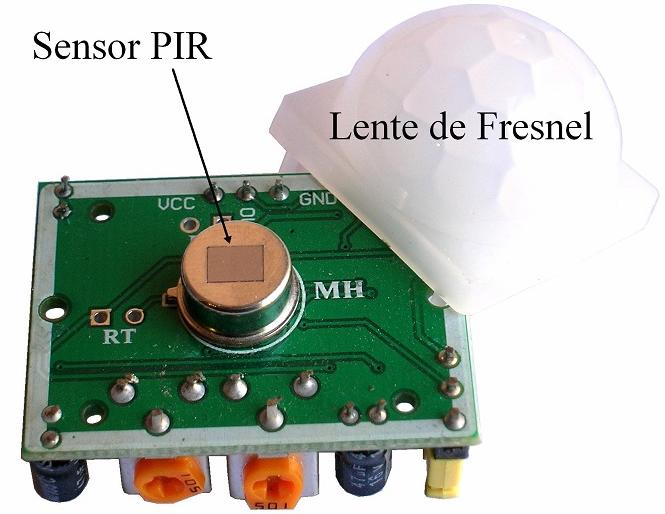
\includegraphics[width=0.5\linewidth]{Imagenes/SENSOR-HC-SR501-1000-M}
\end{figure}

\section{Software}

\subsection{RTOS}

Los sistemas operativos en tiempo real, tienen como parámetro clave al tiempo, ya que en gran variedad de situaciones, por ejemplo, un proceso industrial, se requiere recolectar múltiples datos, los cuales son usados para el control de diversos procesos que deben ser ejecutados en determinados instantes, de no ser así, podría causar desde la mala ejecución de una tarea, hasta un accidente según la delicadeza del proceso.\\ 

Para procesos con nula tolerancia a fallos, se conoce como un sistema en tiempo real duro, muchos de estos sistemas se encuentran en el control de procesos industriales, en aeronáutica, en la milicia y en áreas de aplicación similares. El caso contrario, cuando se tiene cierta permisividad a que muy ocasionalmente existan errores, se conoce como sistema en tiempo real suave, los sistemas de audio digital o de multimedia están en esta categoría. Los teléfonos digitales también son ejemplos de sistema en tiempo real suave. \cite{SO} \\

``Como en los sistemas en tiempo real es crucial cumplir con tiempos predeterminados para realizar una acción, algunas veces el sistema operativo es simplemente una biblioteca enlazada con los programas de aplicación, en donde todo está acoplado en forma estrecha y no hay protección entre cada una de las partes del sistema. Un ejemplo de este tipo de sistema en tiempo real es freeRTOS.  Las categorías de sistemas para computadoras de bolsillo, sistemas integrados y sistemas en tiempo real se traslapan en forma considerable. Casi todos ellos tienen por lo menos ciertos aspectos de tiempo real suave. Los sistemas integrados y de tiempo real sólo ejecutan software que colocan los diseñadores del sistema; los usuarios no pueden agregar su propio software, lo cual facilita la protección. \\

Los sistemas de computadoras de bolsillo y los sistemas integrados están diseñados para los consumidores, mientras que los sistemas en tiempo real son más adecuados para el uso industrial. Sin embargo, tienen ciertas características en común''. \cite{SO}

\subsection{ESP-IDF}

ESP-IDF es el entorno de desarrollo oficial para el ESP32 desarrollado por Espressif System, el cual mediante una serie de comandos específicos escritos en la terminal (en el caso de linux), habilita la configuración del ESP32 en cuanto a su funcionamiento, es decir, permite encender o apagar características como el WiFi, el Bluetooth o realizar particiones de memoria, además de esto, se puede cargar el código por el puerto USB al ESP32, al igual que visualizar la información generada por el ESP32 por el mismo puerto. Este entorno se encuentra construido con diferentes características y APIs, algunas de ellas se mencionan a continuación. \cite{ES}

\paragraph{FreeRTOS:}el framework está desarrollado sobre este sistema operativo de tiempo real, tomando algunas funcionalidades propias, como la tareas y las colas.

\paragraph{Wi-Fi:}el módulo ESP-WROOM-32 posee la capacidad en el hardware para la conexión a una red Wi-Fi, y este software proporciona las librerias y las funcionalidades a fin de realizar dicha conexion y enviar o recibir datos.

\paragraph{Particiones:}el MCU contiene una memoria flash, la cual por medio de este framework se le pueden realizar particiones, dedicadas a almacenar la lista de instrucciones, y también para guardar ciertos archivos. Estas se configuran a través de un fichero csv.

%\paragraph{Consola:}el framework provee una libreria para realizar la programacion de una consola, con el fin de ejecutar diferentes funcionalidades programadas dentro del sistema por el desarrollador.

\paragraph{HTTP Request:}para realizar diferentes peticiones HTTP como las descritas anteriormente, el entorno de desarrollo cuenta con la librería LWIP encargada de realizarlas.

\paragraph{Timers:}este framework provee varias funciones con el objetivo de disponer de los timers de 64 bits que posee el ESP32 y además para configurar sea un timer periódico o de un solo disparo.

\subsection{Proteus}

Proteus combina facilidad de uso con características de gran alcance con la finalidad de ayudar a diseñar, probar y concebir PCB profesionales. Con casi 800 variantes de microcontroladores listos para la simulación directamente desde el esquematico. Además de contar con uno de los paquetes de diseño de PCB profesionales más intuitivas en el mercado y un autoruteo de clase mundial incluido como estándar. \cite{Prot1} \\

Además, es una herramienta muy completa y potente de simulación de circuitos y diseño de PCBs. Dentro de la simulación de circuitos admite componentes pasivos, digitales, analógicos y componentes más complejos como LCDs y motores. Por tanto, se puede realizar casi cualquier cosa, el programa está pensado para que una vez se tenga el circuito diseñado se pueda pasar a una PCB \cite{Prot2}. Adicionalmente los dispositivos que no se encuentren se pueden agregar, ya sea de la página oficial o construyéndolos en el software por medio de las funcionalidades provistas.

\subsection{Lógica de la aplicación web}

Para construir la aplicación web se tiene una lógica basada en un Modelo Vista Controlador (MVC), la función de cada parte de esta arquitectura se puede observar en la Figura \ref{fig:mvc}.\\

\begin{figure}[H]
	\centering
	\caption[Modelo-Vista-Controlador.]{Modelo-Vista-Controlador. [Imagen Propia]}
	\label{fig:mvc}
	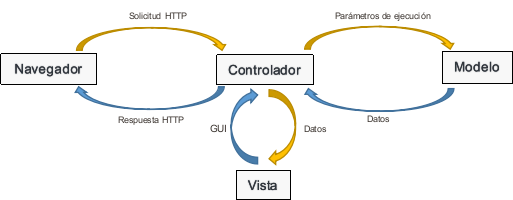
\includegraphics[width=0.7\linewidth]{Imagenes/MVC}
\end{figure}

Su funcionamiento es el siguiente, primero el usuario realiza alguna acción en la interfaz (por ejemplo, presiona un botón, un enlace, etc), luego el controlador recibe (por parte de los objetos de la interfaz-vista) la notificación de la acción solicitada por el usuario. El controlador gestiona el evento que llega, accediendo al modelo y actualizándolo, posiblemente modificándolo de forma adecuada a la acción solicitada por el usuario (por ejemplo, el controlador actualiza los datos del perfil del usuario) y después la interfaz de usuario espera nuevas interacciones del usuario, comenzando el ciclo nuevamente \cite{MVC2}.\\

Este patrón de diseño se usa en la programación orientada a objetos, por lo tanto se realiza la aplicación en el lenguaje de programación PHP, ya que es realmente útil para realizar la gestión de peticiones y envíos de formularios en dicha aplicación, además de que es importante también la gestión de las bases de datos de la aplicación, por este motivo se utiliza un framework basado en este lenguaje y esta arquitectura. Para gestionar las diferentes partes de la aplicación, en este caso se usa el framework Laravel, pues como se menciona anteriormente, está orientado a facilitar las tareas comunes de la mayoría de proyectos web que utilizan HTML5 y PHP.\\

Además, con este framework se hace uso de un ORM (Mapeo Objeto-Relacional) llamado Eloquent. Esta es una forma de mapear los datos que se encuentran en la base de datos a objetos de PHP y viceversa, esto facilita el uso de diferentes gestores de bases de datos como MySQL, SQLite, entre otras, ya que todas las consultas estan en PHP y el ORM ya se encarga del mapeo a los comandos SQL como se observa en la Figura \ref{fig:orm}. Eloquent usa los modelos para enviar y recibir información de la base de datos\cite{Eloq}.\\

\begin{figure}[H]
	\centering
	\caption[ORM]{ORM. [Imagen Propia]}
	\label{fig:orm}
	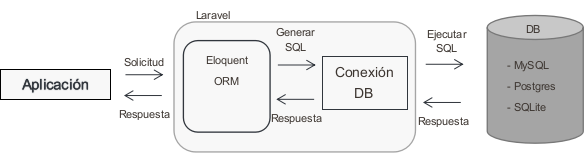
\includegraphics[width=0.7\linewidth]{Imagenes/ORM}
\end{figure}
